
\section{Gesamtpotentiale}
\subsection{Beispiel 1}

	$ V = \pi^{(i)} + \pi^{(a)} $
	
	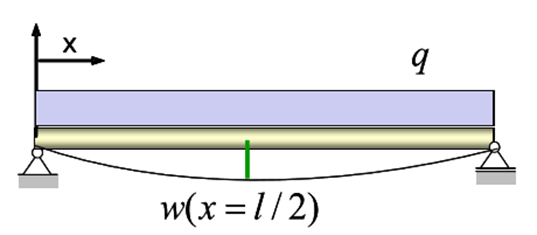
\includegraphics[width=5cm]{potential1}
	
	
\paragraph{ Inneres Potential $ \pi^{(i)} $:}
	\qquad $ V_{Biegung} = \ds\int_{0}^{l} E J\ w''\,^2 \ \dd x $  (Tilde? Dach?)
	
\paragraph{ Äußeres Potential $ \pi^{(a)} $:}
	\qquad $ V_{Kraft} = \pm \dfrac{1}{2}\ F\ w_{(f)} $
	
	Kraft und Verschiebung in verschiedene ($ + $) und gleiche ($ - $) Richtung
	
	$ V_{Streckenlast} = -\ds\int_{0}^{l} \tilde{w}_{(x)}\ q\ \dd x $
	
\subsection{Beispiel 2}

	$ V = \pi^{(i)} + \pi^{(a)} $
	
	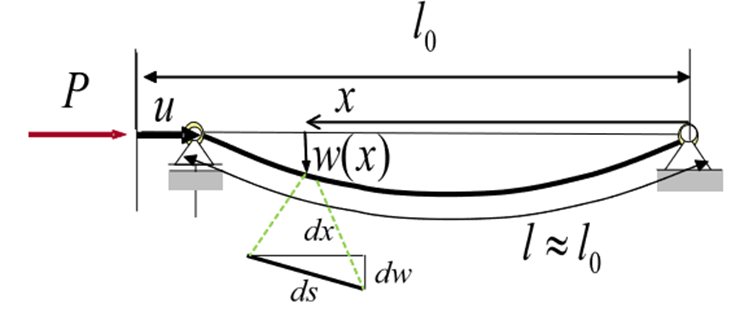
\includegraphics[width=5cm]{potential2}
	
\paragraph{ Inneres Potential $ \pi^{(i)} $}
	\qquad $ V_{Biegung}= \dfrac{1}{2} \ds \int_{0}^{l} E J\ w''\, ^2 \ \dd x $
	
\paragraph{ Äußeres Potential $ \pi^{(a)} $}
	\qquad $ V_{Kraft}  = - P u\approx - P\ \dfrac{1}{2}\ds \int_{0}^{l} w'\, ^2 \ \dd x $
	
\paragraph{	Mögliche Ansatzfunktionen:} \quad 

	Grundsätzlich kann man jegliche Funktion verwenden, aber diese soll der Biegelinie ähneln.
	
	$\rightarrow$ Potenzfunktionen: z.B. $ \varphi_{(x)}=x\ (l-x) $

	$\rightarrow$ Trigonometrische Funktionen: z.B. $ \varphi_{(x)}=\sin{\left(\dfrac{x}{l}\pi\right)} $
	
